%----------------------------------------------------------------------------
\chapter{Evaluation}
%----------------------------------------------------------------------------
This chapter presents the applicability of the designed framework, evaluates its current capabilities and points out improvement possibilities. Section \ref{sec_theoeval} evaluates the current state of the framework, then Section \ref{sec_casestudy} presents a case study about the applicability of our solution. Lastly, Section \ref{sec_futurework} presents the opportunities for the continuation of the work.

%----------------------------------------------------------------------------
\section{Theoretical Evaluation} \label{sec_theoeval}
%----------------------------------------------------------------------------

\clearpage
%----------------------------------------------------------------------------
\section{Case Study: Pedestrian Crossing} \label{sec_casestudy}
%----------------------------------------------------------------------------
This section demonstrates the capabilities and boundaries of the framework. It presents a problem commonly modeled using state-based models, which is complex enough to demonstrate all aspects of the designed Interactive Learning Entity, but also simple enough to solve - thus verify - only using some background knowledge and common sense. [TODO ref gamma tutorial?]

%---------------------------------------------------------------
\subsection{Introduction} \label{subs_casestudyintro}
%---------------------------------------------------------------

The problem to solve is modeling a pedestrian crossing with a standard traffic light and a pedestrian light as illustrated on Figre \ref{fig_casestudy_systemstates}. As the traffic lights and the pedestrian lights on the opposite sides of the crossing behave identically, we are going to model only one instance of each device. 

The traffic light is looping through the red-green-yellow-red sequence. As an extra, there is an interrupted mode that may be triggered by the police, which results in blinking yellow light. The pedestrian light loops through the red-green-red sequence, and turns black when an interrupt arrives. A subsequent interrupt turns the lights back on, also considering that the sytem must always be in a safe state - i.e. the lights must not allow passage for both the pedestrians and the road vehicles at the same time.

\begin{figure}[!ht] 
	\centering
	\fbox{
		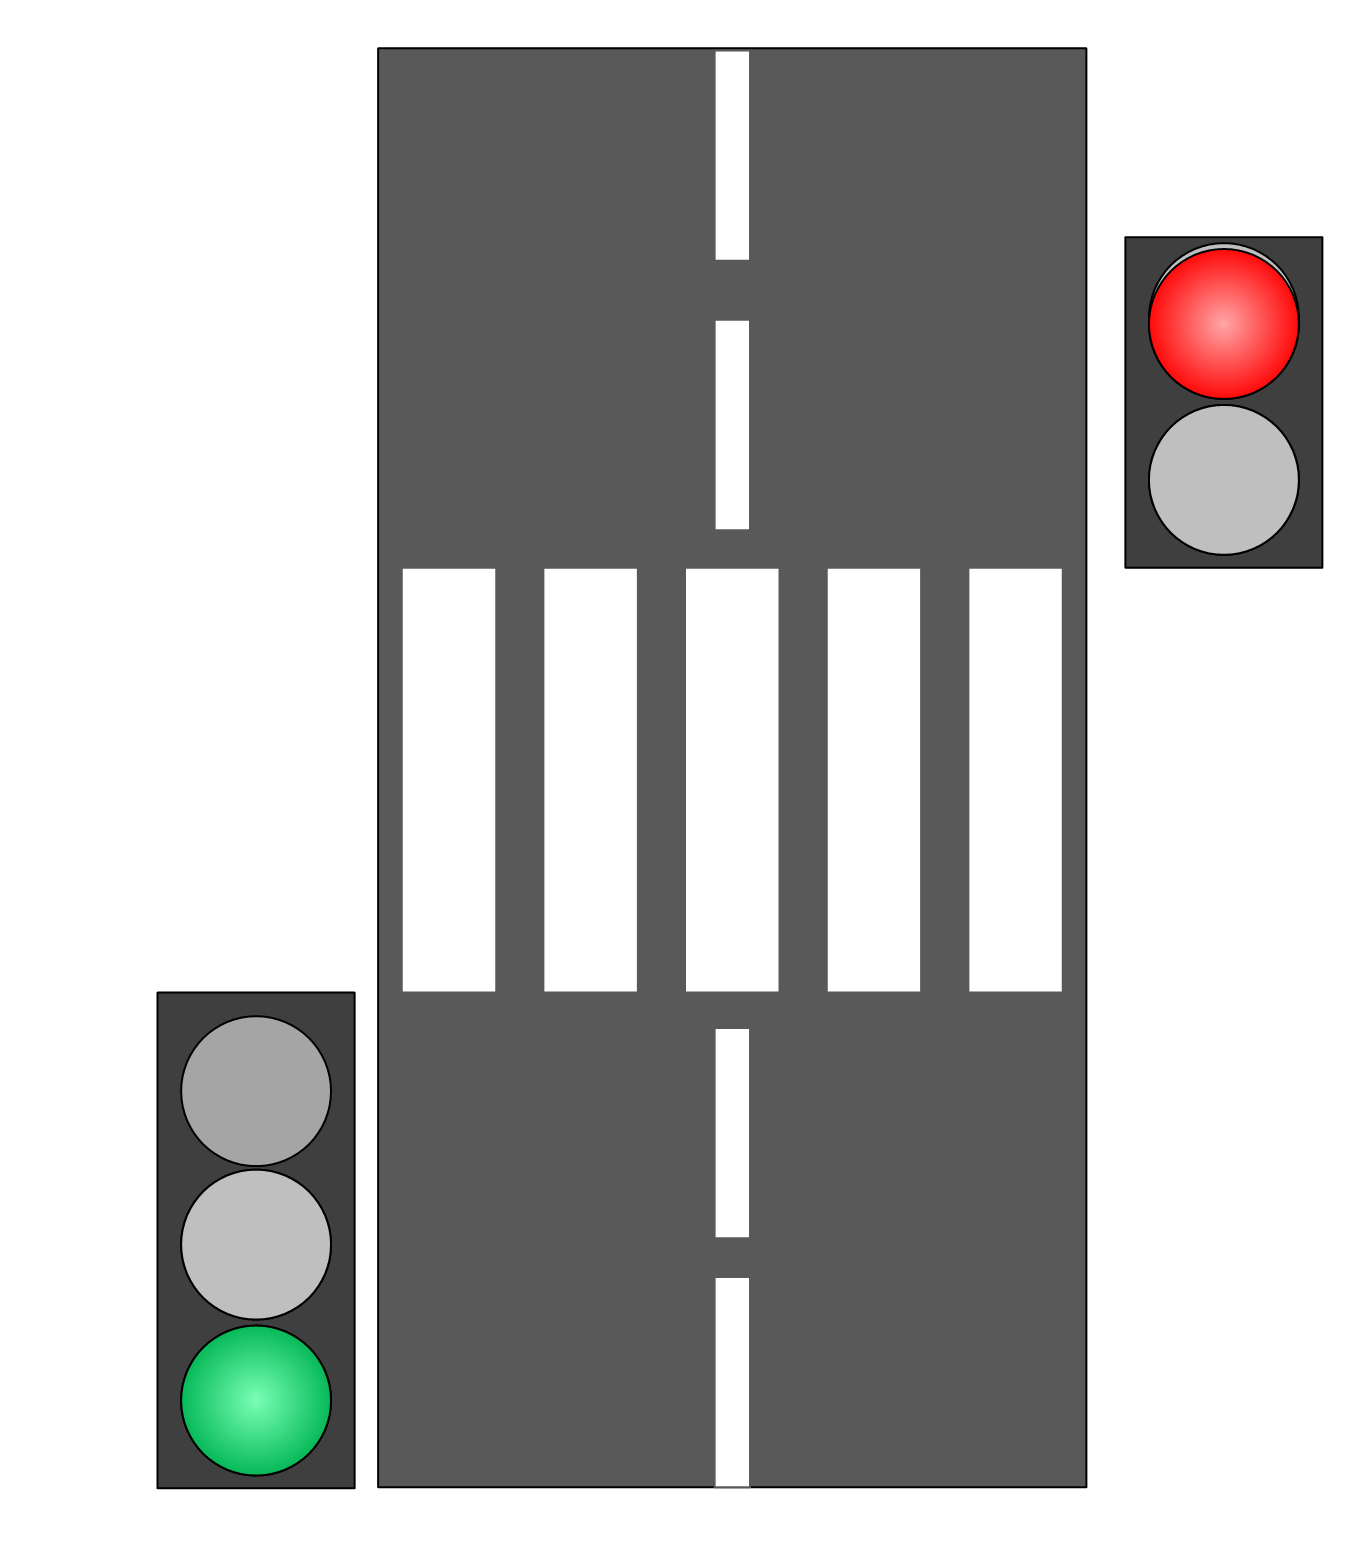
\includegraphics[width=30mm, keepaspectratio]{figures/casestudy_state1.png}
	}
	\fbox{
		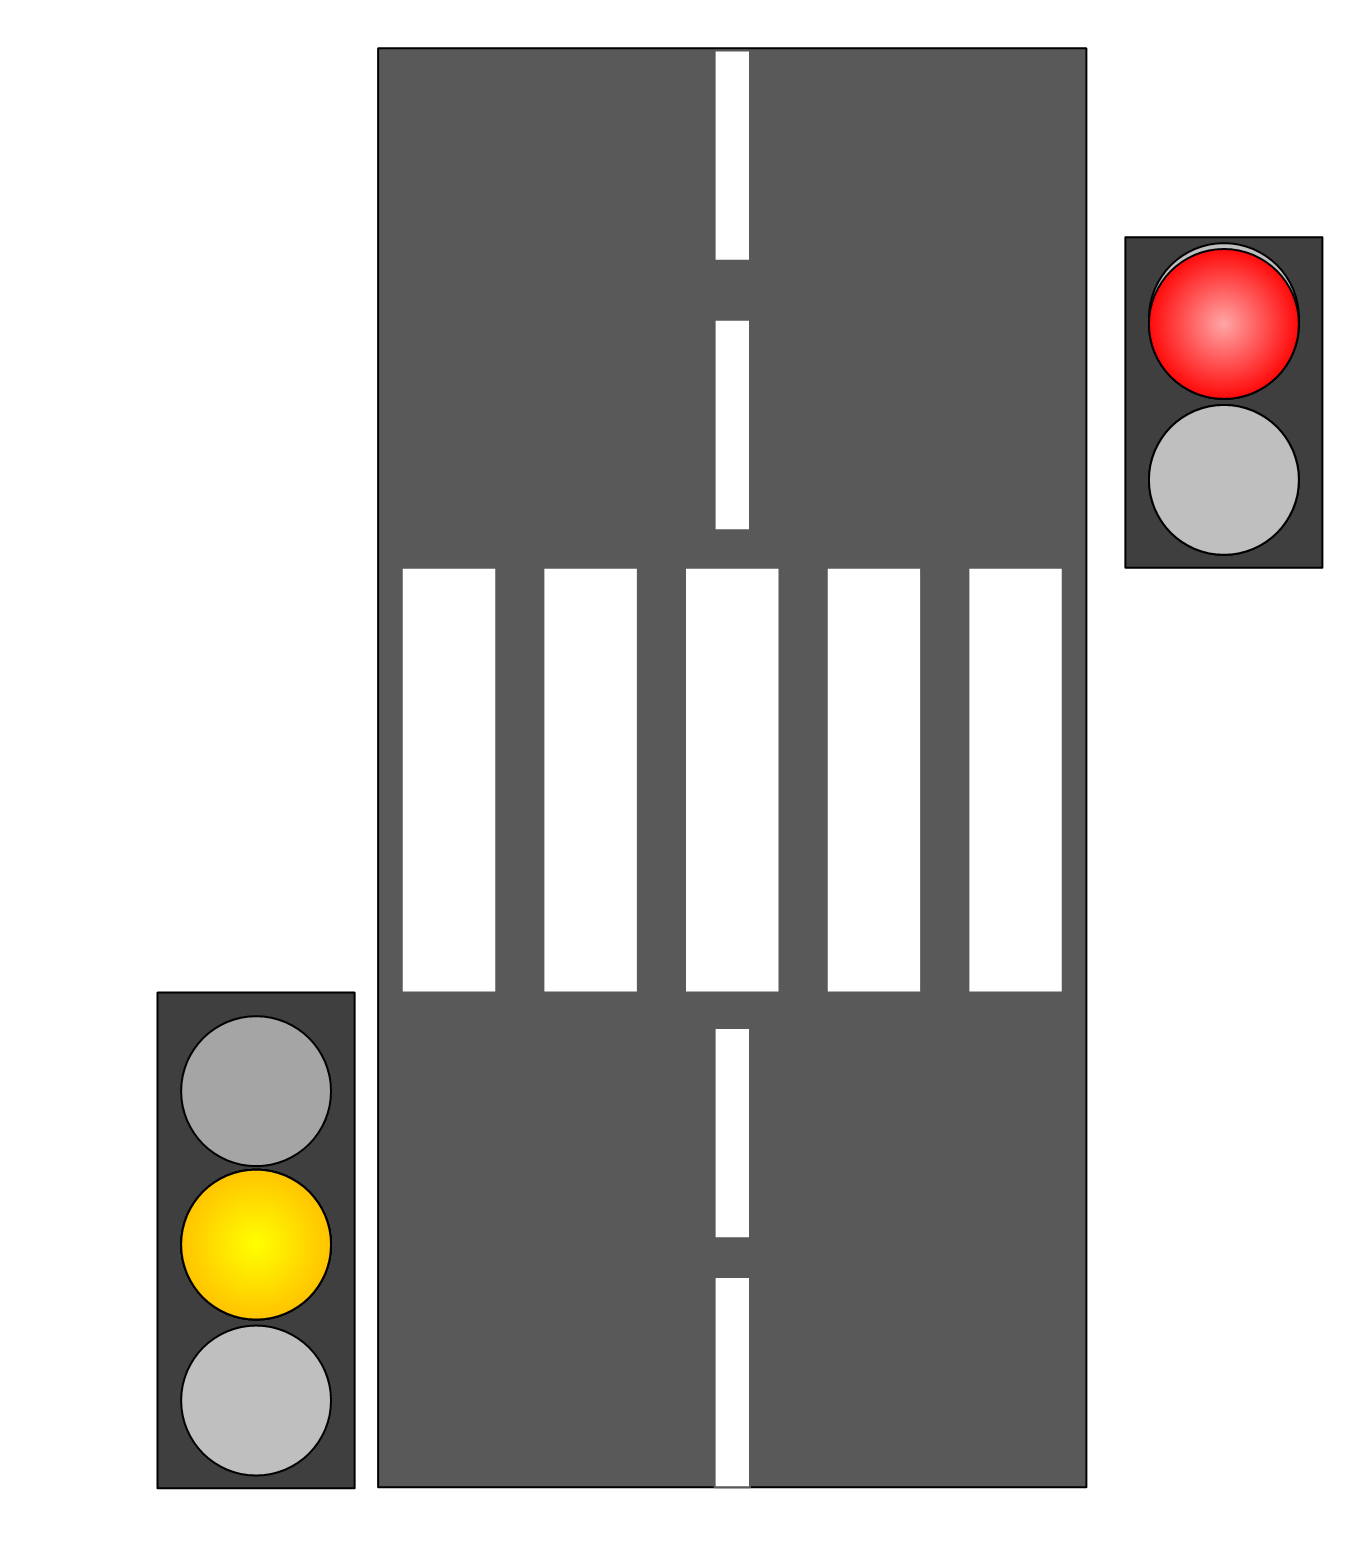
\includegraphics[width=30mm, keepaspectratio]{figures/casestudy_state2.png}
	}
	\fbox{
		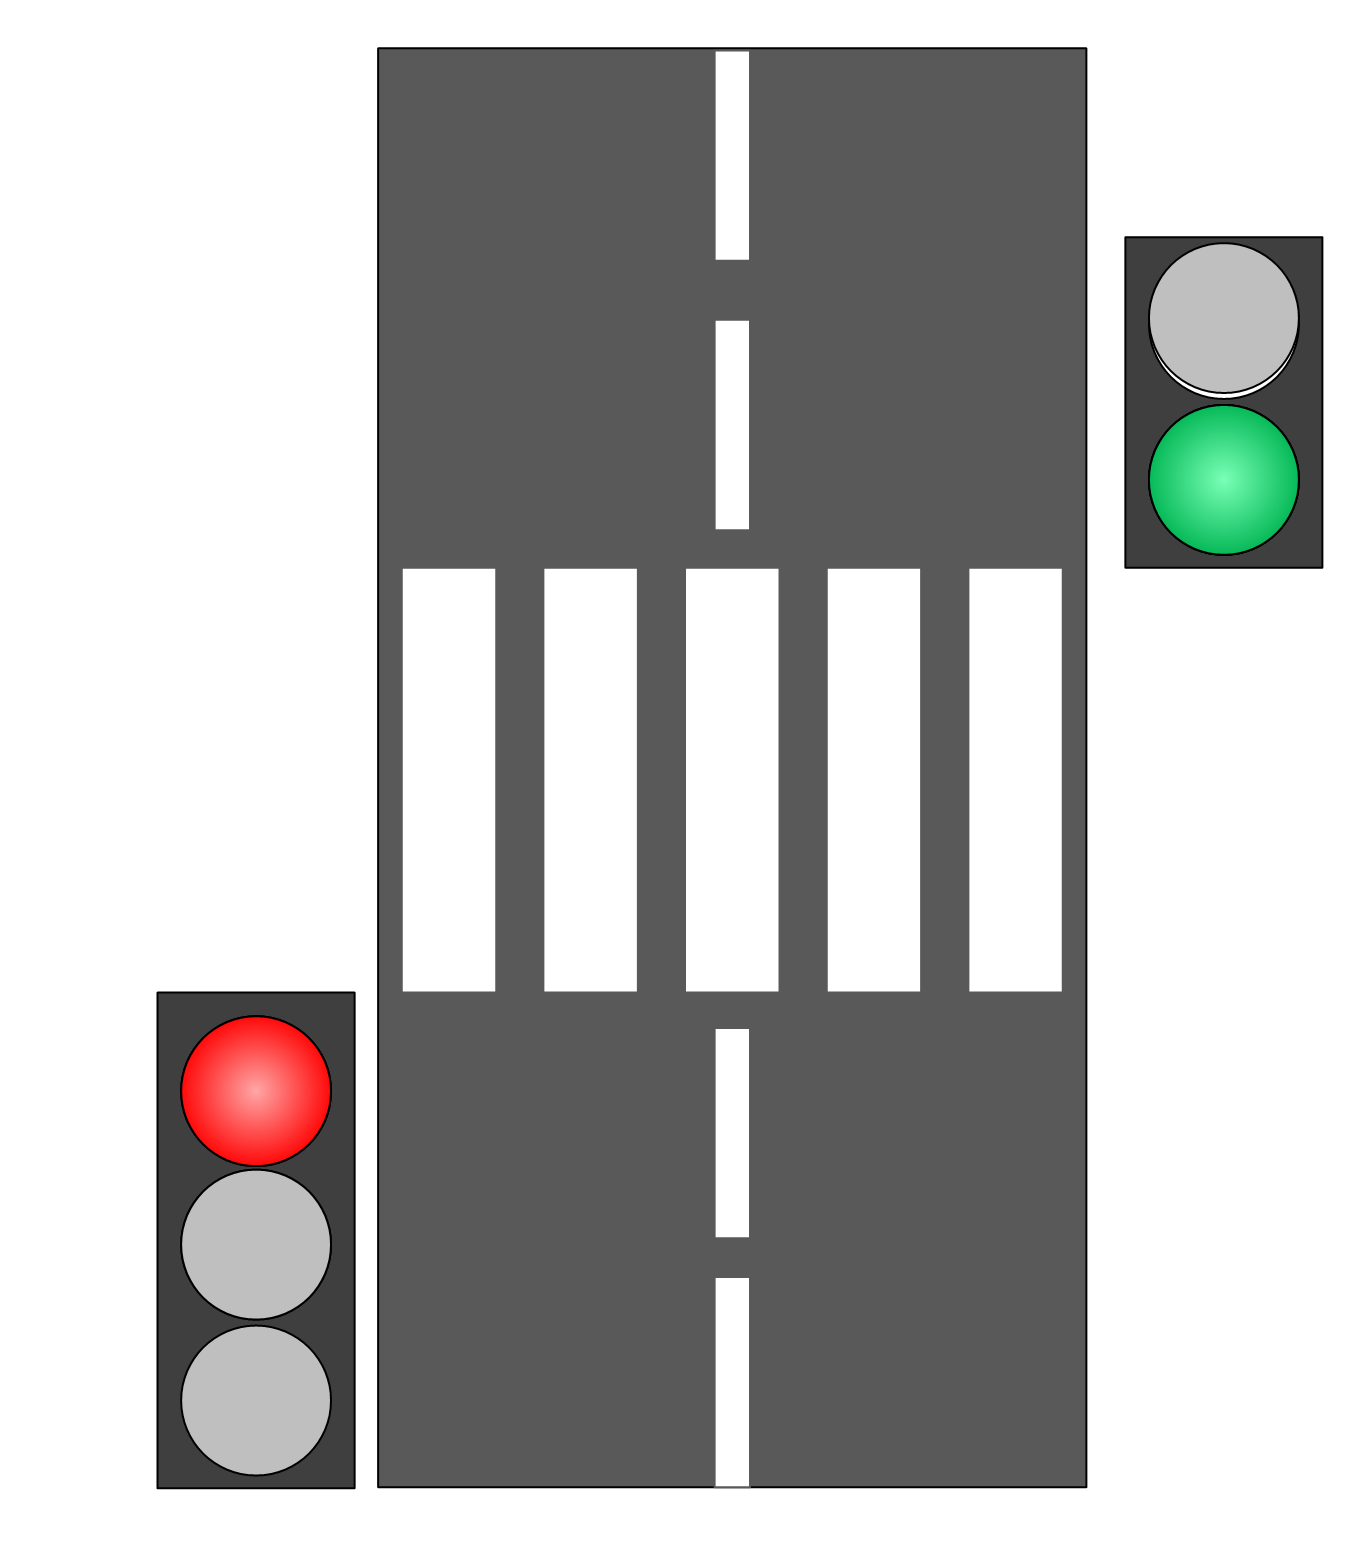
\includegraphics[width=30mm, keepaspectratio]{figures/casestudy_state3.png}
	}
	\fbox{
		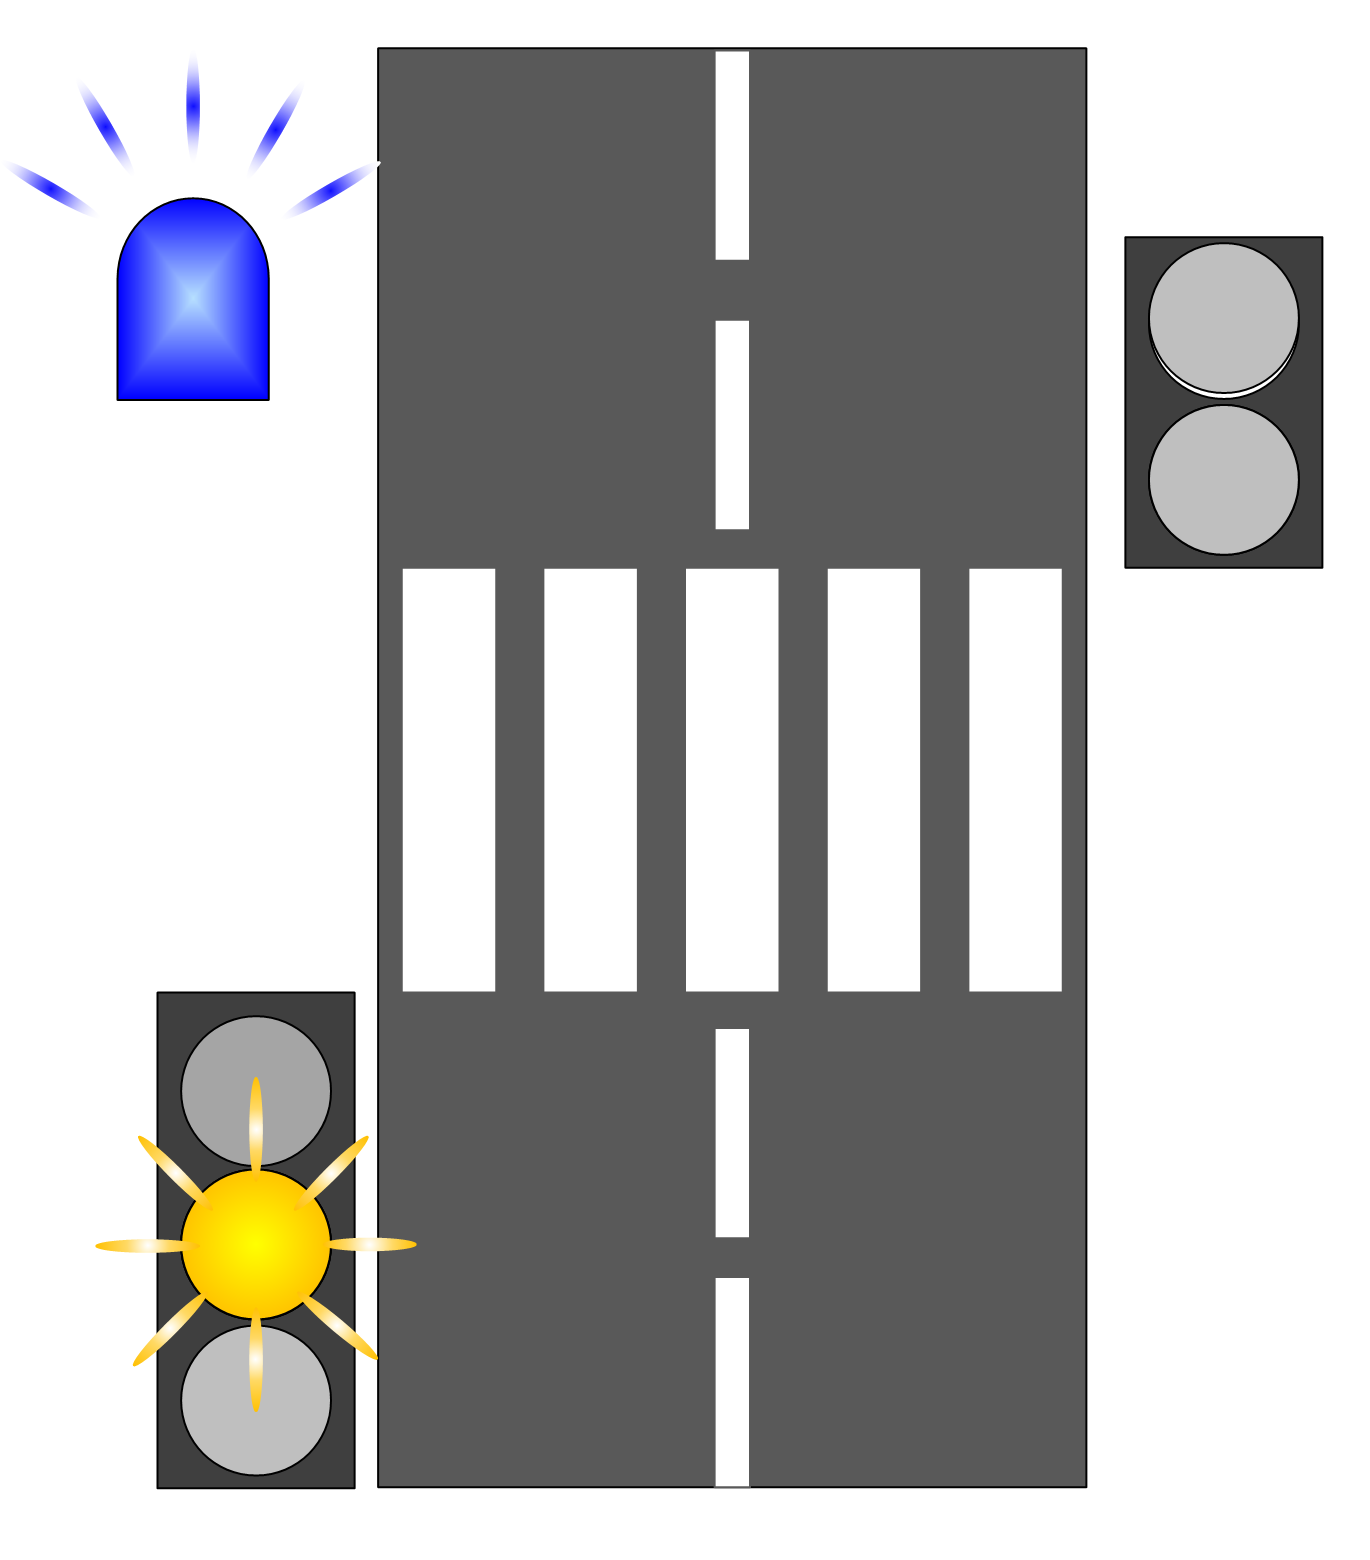
\includegraphics[width=30mm, keepaspectratio]{figures/casestudy_state4.png}
	}
	\caption{Possible states of the system: normal operation (\textit{three from the left}) and the interrupted state \textit{(right)}} 
	\label{fig_casestudy_systemstates}
\end{figure}

%---------------------------------------------------------------
\subsection{Component Design} \label{subs_casestudycomps}
%---------------------------------------------------------------

The previous subsection mentioned two components of the composite system: a traffic light and a pedestrian light. To realize the safe state of the system, the components must synchronize their behavior, justificating the existence of a third, controller component. 

\textbf{The traffic light component} has two inputs on its input interface - toggle and interrupt - and four outputs on its display interface - red, green, yellow and blinking yellow - as it appeared in the problem description.

\textbf{The pedestrian light component} has the same two inputs on its input interface - toggle and interrupt - and three outputs on its display interface - red, green, and black - as it appeared in the problem description.

\textbf{The controller component} controls the rhythm of the change of states and also interrupts the other components when the police interrupt arrives. Thus, it has an input interface for the police interrupt and two output interfaces - matching the inputs of the other components.

The described components and their connections are illustrated on Figure \ref{fig_casestudy_blockdiagram}.

\begin{figure}[!ht] 
	\centering
	%\fbox{
		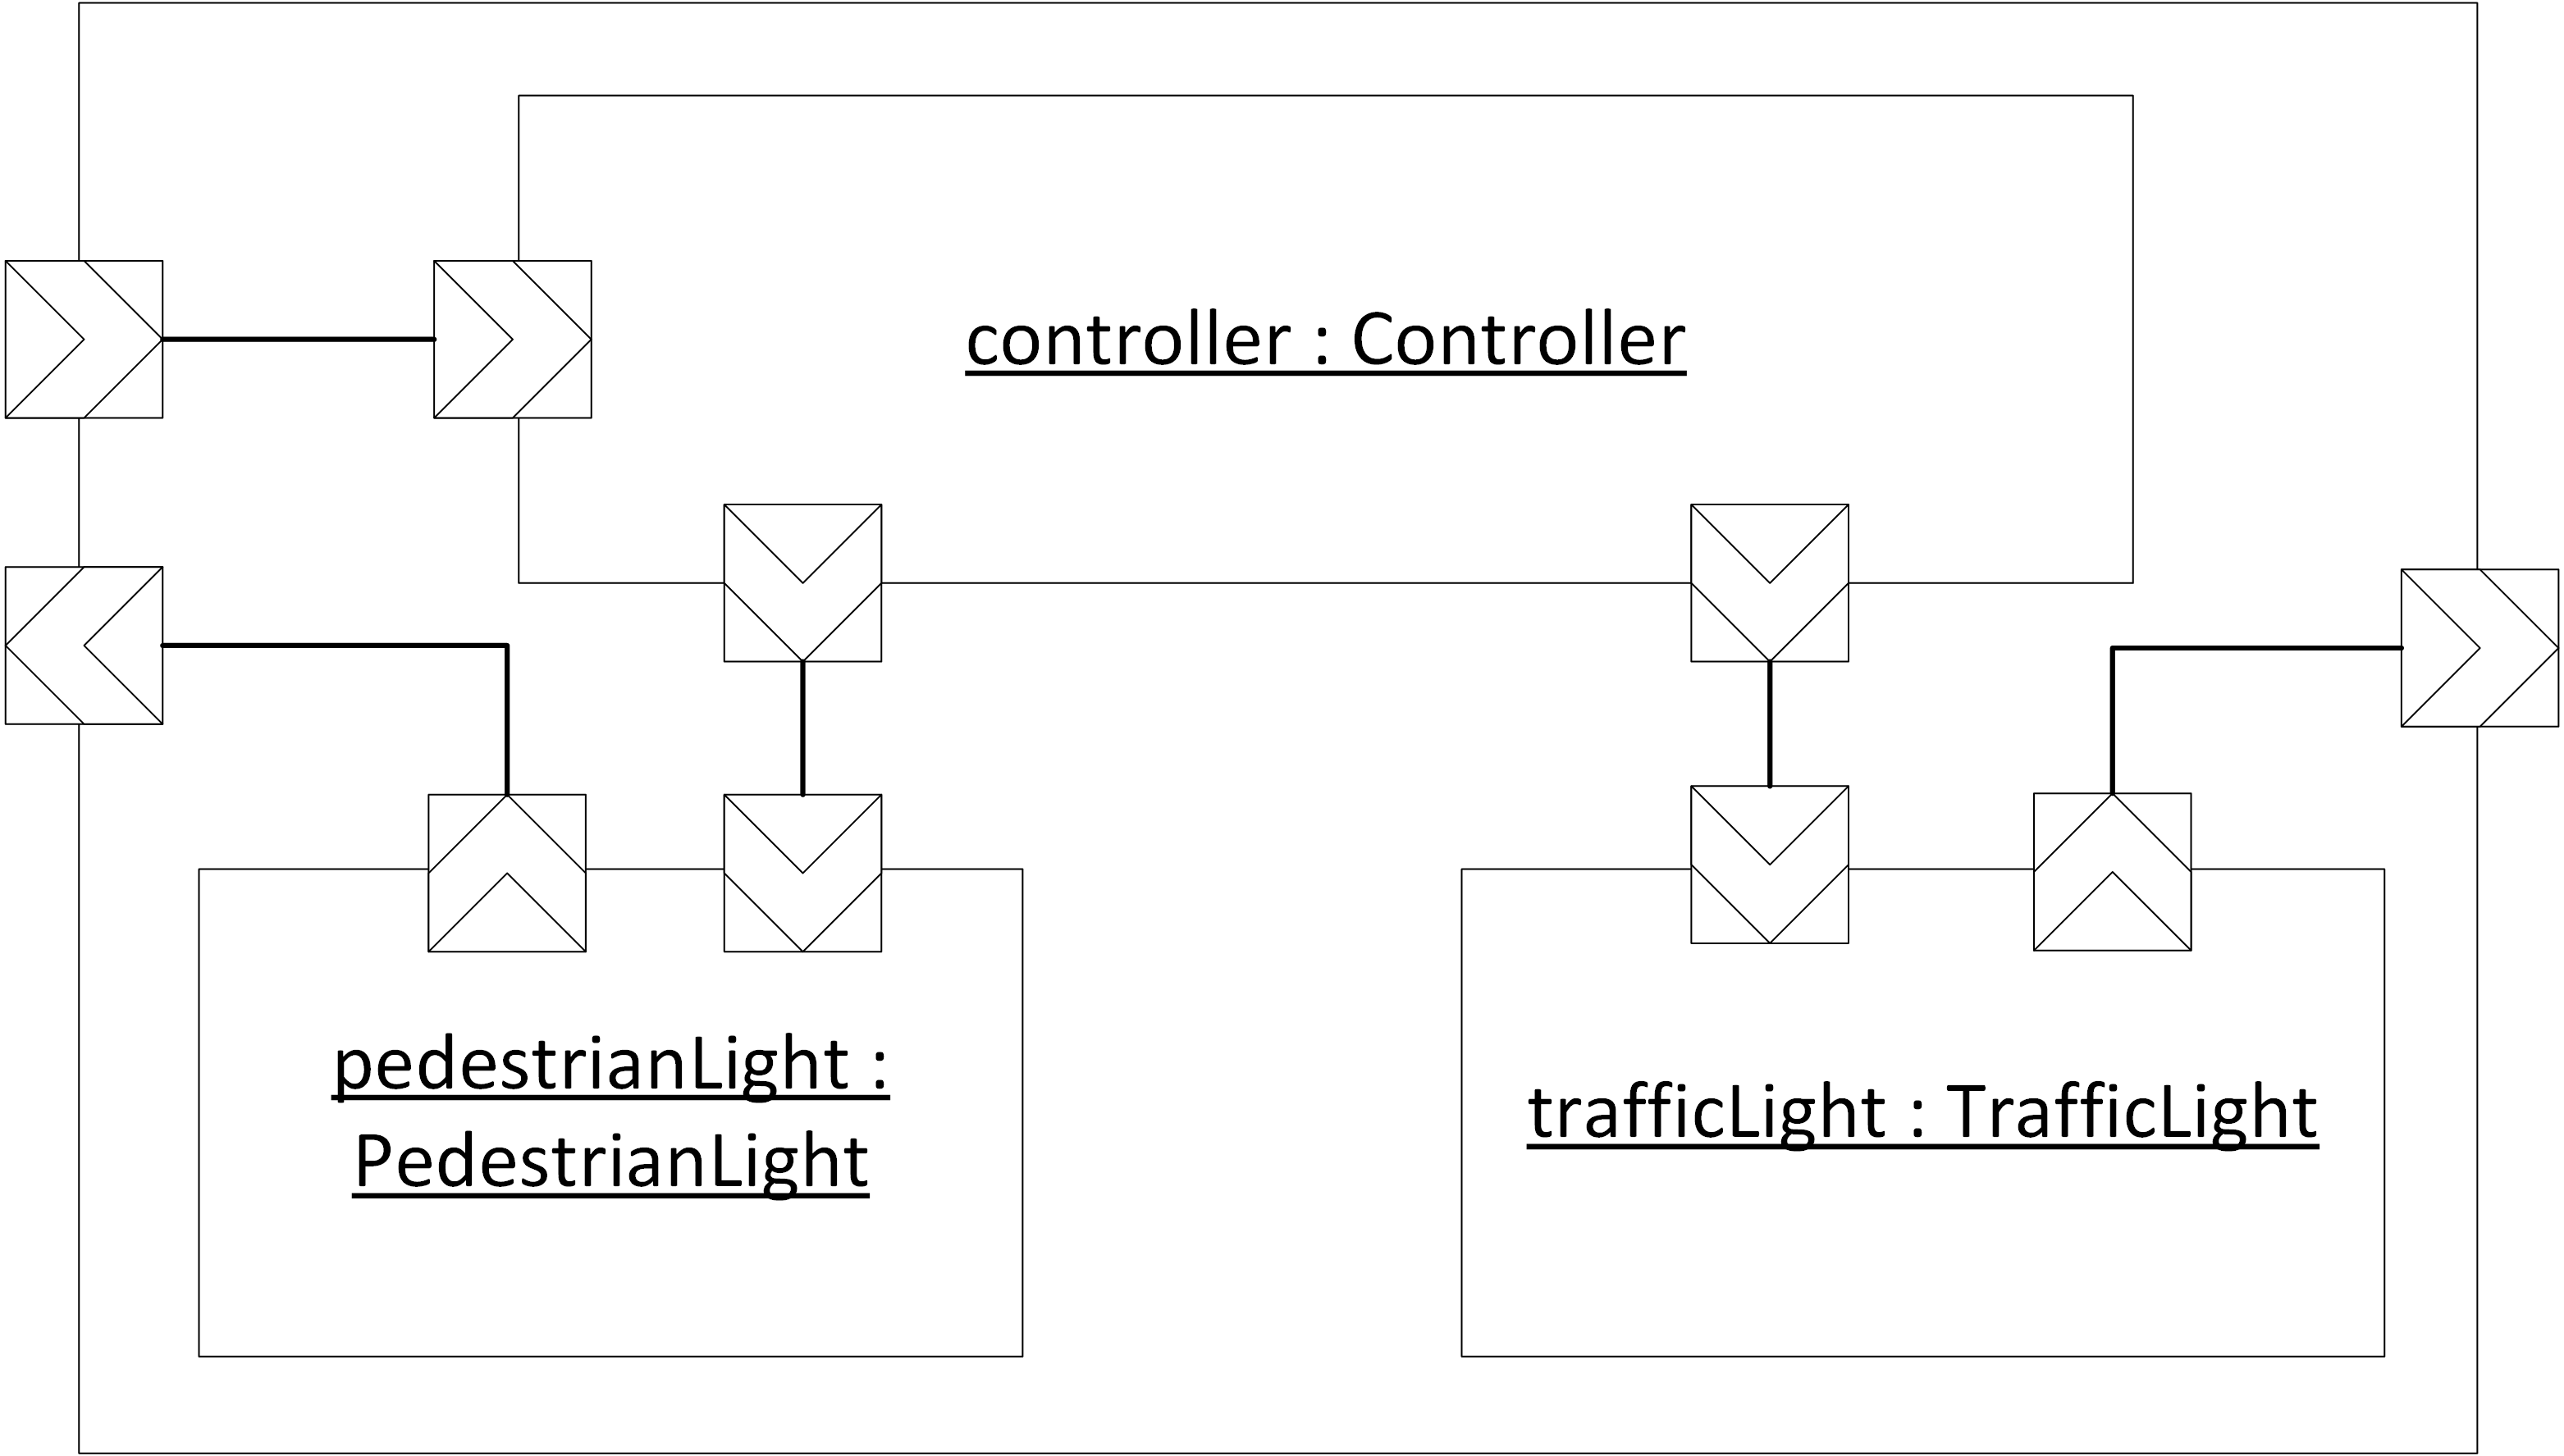
\includegraphics[width=130mm, keepaspectratio]{figures/casestudy_blockdiagram.png}
	%}
	\caption{Components of the modeled system and their connections} 
	\label{fig_casestudy_blockdiagram}
\end{figure}

[TODO interface definitions here]

\textbf{The Expected Behavior of the Components} 

Based on the specification, we expect the traffic light and the pedestrian light components to behave identically to the components illustrated on Figure [TODO]. Naturally, we do not expect the same structure - a statechart with state hierarchy and entry/exit actions - as the current framework is not capable of synthesizing statechart-specific elements. 

[TODO TrafficLight Statechart \& also PedestrianLight here!]

The controller component will be similar with one additional problem. It is not possible to synthesize timeouts to control the rhythm of the toggle signals. For that, we introduce an event not qualified by an interface, which the user can substitute for arbitrary internal logic - e.g. the corresponding timeouts. Thus, we expect a component similar to that on Figure [TODO].

[TODO Controller Statechart!]


%---------------------------------------------------------------
\subsection{Synthesizing the Components} \label{subs_casestudysynth}
%---------------------------------------------------------------

As the components are relatively simple, the algorithm will reach the desired behavior after examining only short traces, resulting in relatively few questions to the user. However, to illustrate the usage of non-trivial requirements formulated in advance, let us define a few LTL expressions, invalid and valid traces for the traffic light component (with the interface qualifications left out for simplicity):

\begin{itemize}
	\item LTL: FG(interrupt -> blinkingYellow | red) meaning that as a result of an interrupt, only blinking yellow or red can be on the output. 
	\item LTL: F(interrupt -> X(G(toggle) -> G(blinkingYellow))) meaning that after an interrupt, if only toggles are the inputs, the outputs are always blinking yellow
	\item Valid Trace: toggle/red toggle/green toggle/yellow toggle/red - the main sequence loop of the traffic light
	\item Invalid Trace: interrupt/green interrupt/green - to enforce the safe state when returning from interrupter
	\item Invalid Trace: interrupt/yellow interrupt/yellow - to enforce the safe state when returning from interrupter 
\end{itemize}

After adding these requirements during the offline phase (qualified with the corresponding interfaces, presented in Listing \ref{lst_exampleofflinefull}), the synthesis of the component can proceed to the online, interactive phase. A possible learning process can be seen in Listing \ref{lst_examplelearning}. In Listing \ref{lst_examplelearningfull} there is a version of this example with logging turned on, so we can infer more about the state of the learning.

\bigskip
\begin{lstlisting} [language=tex,caption=A possible run of the learning process,label=lst_examplelearning]
	Unknown output for input sequence: [trafficControl_interrupt]
	Would you like to specify the output through an (I)O pair, an (L)TL expression, a (V)alid Trace or an I(N)valid Trace?
	>I
	Please provide the expected output:
	>TrafficDisplay.blinkingYellow
	Unknown output for input sequence: [trafficControl_interrupt, trafficControl_interrupt]
	Would you like to specify the output through an (I)O pair, an (L)TL expression, a (V)alid Trace or an I(N)valid Trace?
	>V
	Please provide a valid trace:
	>TrafficControl.interrupt/trafficDisplay.blinkingYellow TrafficControl.interrupt/TrafficDisplay.red TrafficControl.interrupt/TrafficDisplay.blinkingYellow TrafficControl.interrupt/TrafficDisplay.red
	Unknown output for input sequence: [trafficControl_toggle, trafficControl_interrupt]
	Would you like to specify the output through an (I)O pair, an (L)TL expression, a (V)alid Trace or an I(N)valid Trace?
	>I
	Please provide the expected output:
	>TrafficDisplay.blinkingYellow
	Unknown output for input sequence: [trafficControl_toggle, trafficControl_interrupt, trafficControl_interrupt]
	Would you like to specify the output through an (I)O pair, an (L)TL expression, a (V)alid Trace or an I(N)valid Trace?
	>I
	Please provide the expected output:
	>TrafficDisplay.red
	Unknown output for input sequence: [trafficControl_toggle, trafficControl_toggle, trafficControl_interrupt]
	Would you like to specify the output through an (I)O pair, an (L)TL expression, a (V)alid Trace or an I(N)valid Trace?
	>I
	Please provide the expected output:
	>TrafficDisplay.blinkingYellow
	Unknown output for input sequence: [trafficControl_toggle, trafficControl_toggle, trafficControl_interrupt, trafficControl_interrupt]
	Would you like to specify the output through an (I)O pair, an (L)TL expression, a (V)alid Trace or an I(N)valid Trace?
	>I
	Please provide the expected output:
	>TrafficDisplay.red
	Unknown output for input sequence: [trafficControl_toggle, trafficControl_toggle, trafficControl_toggle, trafficControl_interrupt]
	Would you like to specify the output through an (I)O pair, an (L)TL expression, a (V)alid Trace or an I(N)valid Trace?
	>I
	Please provide the expected output:
	>TrafficDisplay.blinkingYellow
	Equivalence Query. Please provide a counterexample if exists.
\end{lstlisting}

The rest of the components can be synthesized in a similar fashion. 

%---------------------------------------------------------------
\subsection{The Resulting Models} \label{subs_casestudyresults}
%---------------------------------------------------------------


%----------------------------------------------------------------------------
\section{Future Work} \label{sec_futurework}
%----------------------------------------------------------------------------

